\documentclass[mathserif,blue]{beamer}
\usepackage[includemp=true,marginparsep=.5cm,marginparwidth=3cm,left=.7cm,right=1.7cm,top=2cm,bottom=1.5cm]{geometry}
\usepackage{amsmath,amssymb}
\usepackage{stmaryrd}
\usepackage{verbatim}
\usepackage{mdwlist}%提供紧凑的列表
\usepackage{graphicx}
\usepackage{tikz}
\usepackage{ifthen}
\usepackage[colorlinks=true,linkcolor=blue,citecolor=blue]{hyperref}
\usepackage{xfrac}%提供斜分数命令,\sfrac{1}{3}
\usepackage{ctex}
%\usepackage{titlesec}%标题格式
\usepackage{fancyhdr}%页眉页脚
\usepackage{listings}%插入代码
\usepackage{framed}
\usepackage{lipsum}
\usepackage{subfig}%子图
\usepackage{tabularx,booktabs}%插入表格
\usepackage{indentfirst} %首行缩进
\usepackage{array} 
\usepackage{longtable}%长表格
\usepackage{multirow}%使用多栏宏包
\usepackage{wrapfig}%文字环绕
\usepackage{extarrows}
\usepackage{ulem,bm}
\usepackage{cite}%参考文献
\usepackage[super,square,comma,sort&compress]{natbib} 
\usepackage{setspace}%设定行距

\setCJKfamilyfont{huawen}{STXihei}
\setCJKfamilyfont{hwzhs}{STZhongsong}
\newcommand\xihei{\CJKfamily{huawen}} %华文细黑
\newcommand\zhongsong{\CJKfamily{hwzhs}}%华文中宋
\usetikzlibrary{arrows,arrows.spaced,arrows.meta,calc,intersections,through,backgrounds,math,angles,shapes}

\newtheorem{theorem}{定理}
\newtheorem{definition}{\hei 定义}
\newtheorem{property}{问题}
\newtheorem{proposition}{猜测}
\newtheorem{lemma}{引理}
\newtheorem{corollary}{推论}

\newcommand\Dd{\displaystyle}\newcommand{\Tt}{\textstyle}\newcommand{\Ss}{\scriptstyle}\newcommand{\Sss}{\scriptscriptstyle}%
\setlength\mathsurround{0.5ex}%数学模式与文本模式混排时留出的间距
\newcommand\an[1][a]{\ensuremath{\{#1_n\}}}%sequence
\newcommand\ud{\mathrm{d}}
\newcommand{\ue}{\mathrm{e}}%正体字母
\newcommand\triabc{\ensuremath{\triangle ABC}}%三角形ABC
\newcommand\cnm[2][n]{\ensuremath{\textrm{C}^{#2}_{#1}}}%组合数
%数学题目编辑
\newcommand\lines[1][1.2]{\,\underline{\mbox{\hspace{#1cm}}}\,}% 填空题的横线
\newcommand\brackets[1][2]{\nolinebreak\hfill\mbox{~(\hspace{#1em})}\\}% 选择题的括号
%扩展命令
\newcommand\qqquad{\qquad\quad}
\def\aside#1{\marginpar{\footnotesize #1}}
%自动编号之最简
\newcommand\numa{\refstepcounter{numi}\thenumi}\newcounter{numi}
\newcommand\numb{\refstepcounter{numii}\thenumii}\newcounter{numii}
\newcommand\numc{\refstepcounter{numiii}\thenumiii}\newcounter{numiii}
\newcommand\numaa{\refstepcounter{numai}\thenumai}\newcounter{numai}[numi]

\newcommand{\question}[1][]{\par\vspace{1ex}\noindent\refstepcounter{numberi}\textbf{\thenumberi.}\ensuremath{#1}}\newcounter{numberi}[subsection]% 每道小题自动编号
\newcommand\quson{\\ \hspace*{1em}\refstepcounter{numberii}\thenumberii)~}\newcounter{numberii}[numberi]% 每道小题自动编号
\newcommand\choice[5][4]{\vspace*{-1em}\begin{tasks}(#1)\task$#2$\task$#3$\task$#4$\task$#5$\end{tasks}\vspace*{-1.2em}}%选择题排版之数学模式
\newcommand\choicex[5][4]{\vspace*{-1em}\begin{tasks}(#1)\task#2\task#3\task#4\task#5\end{tasks}\vspace*{-1.2em}}%选择题排版之数学模式
\newcommand\tbs[1][]{\texttt{\char92#1}}
\newcommand\bpics[1]{\par\vspace{1ex}\noindent\begin{minipage}{\textwidth}\begin{minipage}{#1\textwidth}}
\newcommand\mpics[1]{\end{minipage}\begin{minipage}{#1\textwidth}\linespread{1}}
\newcommand\epics{\end{minipage}\end{minipage}\par\vspace{2ex}}

\newcommand\set[1]{\lbrace\ensuremath{#1}\rbrace}
\newcommand\setx[1]{\{#1\}}

\newcommand\mybf[1]{{\bm#1}}
\def\bfR{\mybf R}
\def\bfN{\mybf N}
\def\bfZ{\mybf Z}
\def\bfQ{\mybf Q}
\def\bfC{\mybf C}
\def\bfZp{\mybf Z^+}

\newcommand\myvec[1]{\bm#1}
\def\veca{\myvec a}
\def\vecb{\myvec b}
\def\vecc{\myvec c}
\def\vecd{\myvec d}
\def\vece{\myvec e}
\def\vecf{\myvec f}
\def\vecs{\myvec e}
\def\vecp{\myvec p}
\def\vecq{\myvec q}
\def\veci{\myvec i}
\def\vecj{\myvec j}
\def\vecei{\myvec{e_1}}
\def\veceii{\myvec{e_2}}
\def\veczero{\myvec 0}
\newcommand\lvec[1]{\overrightarrow{#1}}
%background rectangle/.style={draw=blue!50,fill=blue!20,rounded corners=1ex},show background rectangle

%\begin{columns}\begin{column}{\.5\textwidth} \end{column}\begin{column}{.5\textwidth} \end{column}\end{columns}

%受命于tikz
\def\mystyle{\tikzset{myvec/.style={-stealth}}}
%兼容于beamer
\def\pause{}

%%%listings设置    \begin{lstlisting} !!code!! \end{lstlisting}
\lstset{
        numbers=none, %设置行号位置
       numberstyle=\wuhao, %设置行号大小
        keywordstyle=\color{blue}, %设置关键字颜色
        commentstyle=\color[cmyk]{1,0,1,0}, %设置注释颜色
        %frame=shadowbox, %设置边框格式
        escapeinside=``, %逃逸字符(1左面的键),用于显示中文
        breaklines, %自动折行
        extendedchars=false, %解决代码跨页时,章节标题,页眉等汉字不显示的问题
        xleftmargin=0em,xrightmargin=0em, aboveskip=0.5em,%设置边距
        framextopmargin=0pt,framexbottommargin=2pt,abovecaptionskip=-3pt,
        belowcaptionskip=0pt,  
        %tabsize=1, %设置tab空格数
        showspaces=false %不显示空格
        commentstyle=\color{red!50!green!50!blue!50},%浅灰色的注释  
        keywordstyle=\color{blue!90}\bfseries, %代码关键字的颜色为蓝色,粗体  
        rulesepcolor=\color{red!20!green!20!blue!20},%代码块边框为淡青色  
        numberstyle={\color[RGB]{255,1,1}\scriptsize} ,%设置行号的大小,大小有tiny,scriptsize,footnotesize,small,normalsize,large等  
        numbersep=8pt,  %设置行号与代码的距离,默认是5pt  
  basicstyle=\footnotesize, % 这句设置代码的大小  
        frame=shadowbox, %把代码用带有阴影的框圈起来  
        backgroundcolor=\color[RGB]{245,245,244},   %代码背景色         
       }
%\usepackage[includemp=true,marginparsep=.5cm,marginparwidth=3cm,left=2.5cm,right=2cm]{geometry}%带有旁注marginpar
%\usepackage[paperheight=6in,paperwidth=4.5in,margin=1cm]{geometry}%kindel专用


\begin{document}
\title{向量数乘运算及其几何意义}
\author{王崇宁}
\institute[四中]{郑州四中}
\logo{\threesides}
\maketitle

\begin{frame}{向量运算的定义}
  已知非零向量$\bfa$, $\bfa+\bfa$我们记作$2\bfa$,表示这是两个$\bfa$相加,我们也可以理解为$2$乘$\bfa$. $-\bfa-\bfa$我们记作$-2\bfa$,表示这是两个$-\bfa$相加,我们也可以理解为$-2$乘$\bfa$. 

把这个推广,可以定义$\lambda\bfa$, 起个名字叫做$\lambda$与$\bfa$的数乘积,这种运算叫做\colorwordsa{向量的数乘}运算。 
\end{frame}

\begin{frame}{具体规定}
  设向量$\bfa\ne\mathbf 0$, $\lambda\in\bfR$, 
  \begin{block}{方向}
    当$\lambda>0$时,$\lambda\bfa$与$\bfa$方向相同;\\
    当$\lambda<0$时,$\lambda\bfa$与$\bfa$方向相反;
  \end{block}
  \begin{block}{长度}
    $|\lambda\bfa|=|\lambda||\bfa|$;
  \end{block}
  \begin{block}{补充}
    当$\lambda=0$时,$\lambda\bfa=\mathbf 0$.
  \end{block}
%当$|\lambda|>1$时,模变大;当$0<|\lambda|<1$时,模变小;
%注:运算的对象是一个实数和一个向量,结果是一个向量。
\end{frame}

\begin{frame}{运算的运算律}
  \begin{alertblock}{运算律}
    设$\lambda,\mu$是实数, 
    \begin{center}\begin{itemize}
      \item $\lambda(\mu\bfa)=(\lambda\mu)\bfa$ (结合律);
      \item $(\lambda+\mu)\bfa=\lambda\bfa+\mu\bfa$ (第一分配律);
      \item $\lambda(\bfa+\bfb)=\lambda\bfa+\lambda\bfb$ (第二分配律).
    \end{itemize}\end{center}
  \end{alertblock}
  \begin{exampleblock}{特例}
    \begin{align*}
      (-\lambda)\bfa=-(\lambda\bfa)=\lambda(-\bfa)\\
      \lambda(\bfa-\bfb)=\lambda\bfa-\lambda\bfb 
    \end{align*}
  \end{exampleblock}
%解释一下第三条
\end{frame}

\begin{frame}{小练一题}
  \begin{exampleblock}{计算}
    (1)$(-3)\times4\bfa$\\
    (2)$3(\bfa+\bfb)-2(\bfa-\bfb)-\bfa$\\
    (3)$(2\bfa+3\bfb-\bfc)-(3\bfa-2\bfb+\bfc)$
  \end{exampleblock}
\end{frame}

\begin{frame}{向量共线基本定理}
  \begin{block}{向量共线基本定理}
    向量$\bfa(\bfa\ne\bfzero)$与$\bfb$共线,当且仅当有唯一一个实数$\lambda$, 使$\bfb=\lambda\bfa$.
  \end{block}
  (1)把$\bfb$用向量$\bfa$来表示\\
  (2)判断两个向量是否共线。
\end{frame}

\begin{frame}{一题小练}
  \begin{exampleblock}{例题}
    如图,已知任意两个向量$\bfa,\bfb$, 试作$\overrightarrow{OA}=\bfa+\bfb$, $\overrightarrow{OB}=\bfa+2\bfb$, $\overrightarrow{OC}=\bfa+3\bfb$. 问$A, B,C$三点是否共线。
  \end{exampleblock}
  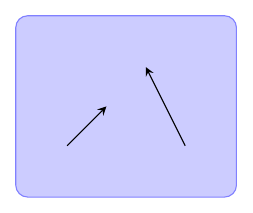
\begin{tikzpicture}[scale=.5,background rectangle/.style=
{draw=blue!50,fill=blue!20,rounded corners=1ex},show background rectangle]
    \clip(0,0)rectangle(5,4);
    \draw[-stealth](1,1)--(2,2)node[left]{$\bfa$};
    \draw[-stealth](4,1)--(3,3)node[right]{$\bfb$};
  \end{tikzpicture}
\end{frame}

\begin{frame}{一题小练}
  \begin{exampleblock}{例题}
    如图,已知任意两个向量$\bfa,\bfb$, 试作$\overrightarrow{OA}=\bfa+\bfb$, $\overrightarrow{OB}=\bfa+2\bfb$, $\overrightarrow{OC}=\bfa+3\bfb$. 问$A, B,C$三点是否共线。
  \end{exampleblock}
  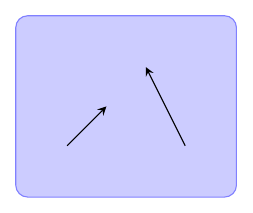
\begin{tikzpicture}[scale=.5,background rectangle/.style=
{draw=blue!50,fill=blue!20,rounded corners=1ex},show background rectangle]
    \clip(0,0)rectangle(5,4);
    \draw[-stealth](1,1)--(2,2)node[left]{$\bfa$};
    \draw[-stealth](4,1)--(3,3)node[right]{$\bfb$};
  \end{tikzpicture}
\end{frame}

\end{document}

\begin{columns}\begin{column}<1->{0.55\textwidth}
  
\end{column}\begin{column}<2->{0.4\textwidth}
  
\end{column}\end{columns}    
